\chapter{16 Tales 2}

\section{Information}

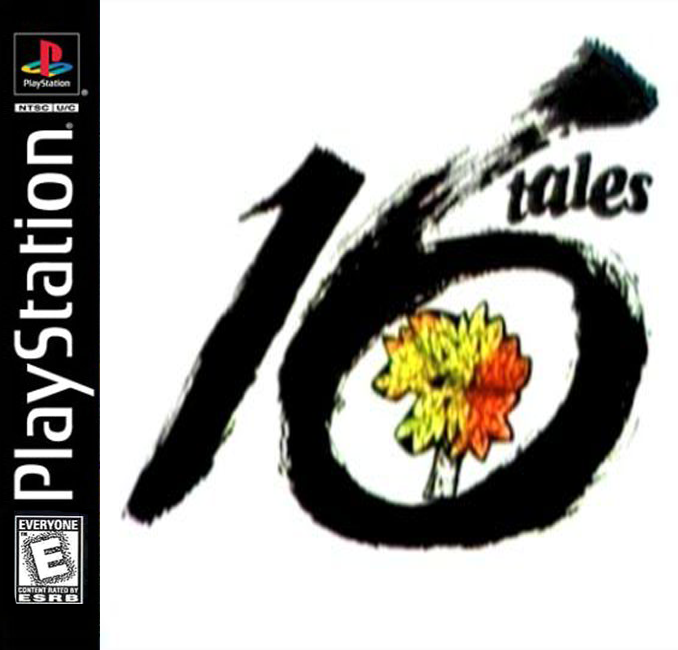
\includegraphics[width=\textwidth/2]{"./Games/16Tales/16TalesGeneralLogo.png"}

The second of the four 16 Tales games published and released by The Lightspan Partnership for the PlayStation 1. Each game consists of four 15-minute video programs various cultures' stories and lore.

16 Tales 2 features a series of four Native American stories, including:
\begin{itemize}
    \item The Blind Man's Daughter
    \item Jose and the Croocodile
    \item Ma Liang and the Magic Brush
    \item The Tale of Urashima Taro
\end{itemize}

Music used throughout:
- Sun Valley by David Snell

\begin{table}[h]
    \centering
    \begin{small}

        \begin{tabular}{|p{1.5cm}|p{8.5cm}|p{7cm}|}
            \hline
            \textbf{Story Title} & \textbf{Short Description} & \textbf{Credits} \\
            \hline
            The Blind Man's Daughter
                                 &
            This story comes from Korea. The story revolves around Shim Cheong, a dutiful daughter living with her blind father.
            To restore her father's sight, she sacrifices herself to a river dragon in exchange for 300 bags of rice that could cure him.
            Shim Cheong is taken to the dragon's palace where she lives in comfort.
            Eventually, she emerges from a lotus blossom, catches the attention of the king, and becomes his wife.
            Despite her newfound happiness, Shim Cheong's thoughts remain with her father, whom she eventually finds and restores his sight.
            The story highlights Shim Cheong's selflessness, sacrifice, and eventual reward for her devotion to her father.
                                 &
            Told by: Hyun-Oak Alan Kim,
            Producer: K. Hamamura Nelson,
            Executive Producer and Director: Edmond R. Chavanette,
            Story Editor: Suzie Kim Oh,
            Illustrator: Hee Do Cho,
            Titles and Set: Doug Stiles,
            Lighting: Ron A. Vanicek,
            Technical Director: Bill Bolle,
            Audio: Larraine E. Wilson,
            Video: Roger Knipp,
            Videotape: Clarence Pemberton,
            Camera: John C. Merritt, Martin Miller, Ron A. Vanicek,
            KLCS Los Angeles Unified School District
            \\
            \hline
            Jose and the Croocodile
                                 &
            This story comes from the Philippines. The story "Jose and the Crocodile" tells of a young boy named Jose who encounters a crocodile trapped in a net while gathering coconuts.
            Despite the crocodile's plea for help, Jose frees him, hoping for a reward.
            However, the crocodile betrays Jose and tries to eat him, forcing Jose to seek help from passing objects in the river.
            Each object refuses to help, citing ingratitude from humans. Finally, a monkey comes to Jose's rescue, allowing him to escape the crocodile's grasp.
            In gratitude, Jose promises to plant banana trees for the monkey's family.
            This story highlights themes of gratitude, betrayal, and unexpected kindness, typical of Filipino folktales.
                                 &
            Told by: Patricia Payuyo,
            Producer: K. Hamamura Nelson,
            Executive Producer and Director: Edmond R. Chavanette,
            Story Editor: Rolando A. Santos, PhD.,
            Illustrator: Don M. Dumandan,
            Titles and Set: Doug Stiles,
            Lighting: Ron A. Vanicek,
            Technical Director: Bill Bolle,
            Audio: Larraine E. Wilson,
            Video: Roger Knipp,
            Videotape: Clarence Pemberton,
            Camera: John C. Merritt, Martin Miller, Ron A. Vanicek,
            KLCS Los Angeles Unified School District
            \\
            \hline
            Ma Liang and the Magic Brush
                                 &
            This story comes from China. The story tells of a poor peasant boy named Ma Liang who dreams of painting but cannot afford brushes.
            Through hard work and dedication, he practices drawing with makeshift tools until one day, a wizard appears and gifts him a magic brush.
            With this brush, anything he paints becomes real. Ma Liang uses his brush to help his village by painting clothes, animals, and food for the needy.
            However, when the greedy Emperor hears of Ma Liang's brush, he seeks to use it for his own gain.
            Ma Liang outwits the Emperor and continues to use his brush for good, traveling across China to help those in need.
            The story showcases themes of kindness, perseverance, and the power of creativity.
                                 &
            Told by: Jeanne Joe,
            Producer: K. Hamamura Nelson,
            Executive Producer and Director: Edmond R. Chavanette,
            Story Editor: Janna R. Wong,
            Illustrations: Castelar Elementary School,
            Titles and Set: Doug Stiles,
            Lighting: Ron A. Vanicek,
            Technical Director: Bill Bolle,
            Audio: Larraine E. Wilson,
            Video: Roger Knipp,
            Videotape: Clarence Pemberton,
            Camera: John C. Merritt, Martin Miller, Ron A. Vanicek,
            KLCS Los Angeles Unified School District
            \\
            \hline
            The Tale of Urashima Taro
                                 &
            This storm comes from Japan. "The Tale of Urashima Taro" is a cherished Japanese folk tale that recounts the story of a young fisherman named Urashima Taro.
            Living in a coastal village with his elderly parents, Taro is known for his kindness and skill as a fisherman.
            One day, after a disappointing catch, he rescues a sea turtle from children's torment.
            In gratitude, the turtle, who is actually a princess in disguise, takes Taro to the Dragon Palace under the sea.
            There, he experiences incredible beauty, hospitality, and enchantment, but eventually feels homesick.
            Despite the princess's pleas, Taro decides to return home. Before leaving, she gives him a mysterious lacquered box with strict instructions not to open it.
            Upon his return to the village, Taro finds everything changed and realizes that centuries have passed.
            Feeling lost and lonely, he finally opens the box, which releases a mist that ages him instantly.
            The story explores themes of kindness, the passage of time, and the consequences of curiosity.
            It's one of many beloved folk tales from Japan, sharing valuable lessons and captivating readers with its enchanting narrative.
                                 &
            Told by: David Hirokane,
            Producer: K. Hamamura Nelson,
            Executive Producer and Director: Edmond R. Chavanette,
            Story Editor: Peggy Okeya,
            Illustrations: Kellene Adachi Coy,
            Titles and Set: Doug Stiles,
            Lighting: Ron A. Vanicek,
            Technical Director: Bill Bolle,
            Audio: Larraine E. Wilson,
            Video: Roger Knipp,
            Videotape: Clarence Pemberton,
            Camera: John C. Merritt, Martin Miller, Ron A. Vanicek,
            KLCS Los Angeles Unified School District,
            \\
            \hline
        \end{tabular}
    \end{small}

\end{table}

\clearpage
\newpage

\section{Transcriptions}

\subsection{The Blind Man's Daughter}

Our story today comes from Korea, a country in eastern Asia. In today's story about the blind man's daughter, you will notice that the girl's name is Shim Cheong. "Chun" is her first name, like Jenny or Maria, and "Shim" is her family name. As in many Asian cultures, the family name is set first. So, if your name is John Smith in Korea, you would be called Smith John. Listen now to the tale of "The Blind Man's daughter".

Five hundred years ago, maybe more, there lived in a certain village a girl named Shim Cheong. Her mother had died long ago, and now her father was going blind. Shim Cheong was very beautiful. Her face was smooth and white, her hair was shiny and black. She was very good and honest, and she had never been sick. It was as if nothing could harm her. She guided her father when he had to work, but his blindness kept him from work, and little by little, all they owned had to be sold to keep them alive.

The old man, Shim, became a beggar. He felt ashamed that his daughter had to go with him to beg for coins. One day, he went out alone. He tripped and fell into a ditch. He tried to climb out, but he couldn't. Then, a strong hand reached out and lifted him up, and a voice spoke to him, "Give me 300 bags of rice for the temple, old man, and in time, you shall have your eyes once again." It was the voice of a priest from the temple, and the old man's heart filled with hope.

That evening, he told his daughter what had happened. But as he told her, his hope went away, and he got very, very sad. "I go, I go, there is no way for beggars like us to get so much rice." That night, as Shim Cheong drifted off to sleep, she sighed, "What to do, what to do?"

"As I say," someone answered in a dream. A dead mother told her how to get the rice and help her father see again. The next morning, Shim Cheong awoke early. She dressed in a long grey gown and a big hat. Then, she walked to the house of a very rich merchant. Now, this merchant owned many, many boats. They brought rice to faraway China. But there was a river dragon who would not let the boats go through. He would spit water and lash the waves with his tail. It was too dangerous for boats to sail.

"What must I give you? What must I do so my boats may go through?" said the merchant to the dragon.

"You must bring me a beautiful girl," the dragon answered.

And so, the merchant spread the news far and wide. He'd offer 300 bags of rice to the girl who would give herself to the dragon. Shim Cheong told the merchant that she wished to offer herself to the dragon.

"You do not deserve to die. You are a good daughter and you are dutiful to your father," but there was no other way for Shim Cheong to get the rice. So, the bargain was made.

The next day, Shim Cheong watched the horses carry the bags of rice to the priest's temple. Then, she bowed before the tomb of her mother and prayed, "O heavenly spirits, care for my father until he is cured." And she spoke to her neighbors, "All kind neighbors, care for my father until he's cured." Then, she set forth to keep her part of the bargain.

She wore a beautiful gown of green and red with jewels and golden ribbons in her hair. Her beauty shone brighter than the sun in the eastern sky. Soon, they came to the place in the river where the dragon lashed his huge tail. It was time to sacrifice Shim Cheong to the dragon. The merchant wanted to save her.

"O river dragon, do not take this girl," but the river dragon demanded the beautiful girl. So, Shim Cheong said goodbye to the merchant. She closed her eyes and jumped off the sides of the boat and disappeared into the water.

Instantly, the river became calm and quiet like a garden pool. Shim Cheong floated through the water. Pearls flashed before her eyes. Big, rainbow-colored fish danced by, and sea plants tickled her nose as she brushed past them. At last, she arrived at the palace of the dragon.

"Kind sir, I am the daughter of the blind beggar, Shim. I'm not worthy to come before one so important as you," the river dragon spoke.

"A message has come to us from Hananim, the emperor of heaven and earth. You shall be rewarded for your goodness to your blind father," then, sea maidens dressed Shim Cheong in the finest clothes. They gave her the softest sleeping mats and the richest food.

In this life of comfort and ease, Shim Cheong grew more beautiful than ever. Then one day, the maidens took her to a giant lotus blossom that lay on the river bottom, and they put her right in it. It was so large that it covered her completely.

"Goodbye, Shim Cheong," said the river dragon.

"Goodbye," Shim Cheong answered back, and soon she felt herself rising like a bubble up through the water. When she reached the top, she was floating next to the boat of the rice merchant. But the rice merchant did not see her. All he saw was the blossom.

"Never in heaven or on earth was there such a lotus flower as this," said the merchant. "Let us take it to the king." The merchant presented the flower to the king. The king was delighted. No one else in all the world had such a blossom. Every day, he admired it floating in the garden pool.

All day long, Shim Cheong hid inside the giant flower. Then one night, as she ventured out of the blossom, the king discovered her. She ran to hide, but the blossom had disappeared. The king looked at her, "Can this be a spirit? She's so beautiful." He called his wise men. On the day the lotus flower was brought to the king, a bright new star had appeared in the sky.

"That's a good sign," and so he made Shim Cheong his wife. Shim Cheong was happy in her life as a queen, but some days she would think of her poor father, "Here I have all I want, but my father's eyes are closed to the world."

One day, the king saw her weeping, "Go, my husband," Shim Cheong said to the king. "I have had a dream about a blind man. It makes me cry. I should like to do something for all the blind people in the kingdom." So, a message was sent to all the blind beggars of the kingdom to invite them to a feast in the king's courtyard.

One day, two days, and three days passed. Beggars came from far and near to eat rice and kimchi. Queen Cheong watched every day, hoping the next person would be her father. The end of the feast came, and still no father. Then one day, there was a noise in the courtyard. A latecomer was being pushed about by the servants.

"Father, father, it is my dear father! Let him stay!" She ordered her servants to dress him in new clothing and bring him to her chamber.

"What wonder is this?" said the old man, Shim, when he heard his daughter's voice. "Do apricots bloom in the snow? Do horses have horns? Do dead men come to life? How can I be sure you are truly Chung?" And he rubbed his eyes. Suddenly, just as the temple priest had promised, the old man's sight returned.

"Oh, my goodness, you are beautiful!" he said. The king welcomed the Shim Cheong's father into the palace, and Queen Cheong was happy all day long. Her father could see again. This was the heavenly reward to the dutiful daughter of the blind beggar, Shim.

The story of the blind man's daghter, Shim Cheong, is just one of the many folk tales from Korea. You can find others in your school or public library: stories such as "The Man Who Lived a Thousand Years" and A Korean Cinderella, "Kongjwi and Patjwi". Read and enjoy the folk tales from Korea and from all over the world. Share a story with a friend, so our tales will never end.

\subsection{Jose and the Crocodile}

Long ago, the early people of the Philippines made up stories to tell their children. These folktales were the textbooks of their day. They served to preserve the history and traditions of the people. They told about events that had happened and also tried to explain the interesting things in nature that they saw about them. In a land of volcanoes, earthquakes, and violent storms, there was a lot to try to explain.

Mountains erupted, and sometimes the earth shook beneath their feet, and new islands rose unexpectedly from the sea. The people were always surrounded by nature, so they were often puzzled by some of the oddities they saw. What was this fish with no bones or scales and looked like a blob of jelly? What made insects glow in the dark? Where did the eagle come from and the crocodile? They made up a story for everything. Talking animals are found as characters in folktales everywhere, and as is proper in a tropical country, it is a quick-thinking monkey who is a hero of today's story. "Jose and the Crocodile", and its characters, setting, and topic is a typical Filipino story. This story may be like some stories you have heard before. Tell me if it is. Now listen to this tale of "Jose and the Crocodile".

Jose lived with his family in a little village next to a river. Jose's father raised coconuts, bananas, and other fruits and vegetables. One day, his mother asked, "Jose, will you please gather some coconuts? I need them for cooking and feeding the hogs, and your father would like to sell some at the market.

"Yes, mother, right away," Jose answered.

Jose hitched the water buffalo to a sled. He took his sharp bolo and strapped it to his waist. He climbed on the water buffalo and started looking for fallen coconuts. Jose was too small to climb the tall coconut trees, so he gathered ones that had fallen off the trees. There were not too many on the ground near the house that day, so he wandered farther and farther away. It was hard work, and Jose traveled far. The air was hot and humid. Jose and the water buffalo became very tired and thirsty, so they went to the river for a drink and a quick swim in the cool water.

While Jose was splashing water on the water buffalo, he heard a groan coming from far away. It sounded like a cry of some animal in pain. Jose became worried. He jumped on the water buffalo and rode towards the sound. The groans became louder and louder as they rode. Soon, Jose saw a big rope hanging from a branch of a large tree. At the end of the rope was a net, and in the net, a big crocodile was fighting to get out.

"Hmm, crocodile catchers were here again," thought Jose to himself. "They will make shoes and belts and bags out of this poor crocodile's skin."

"Little boy, please help me. I have a wife and children," begged the crocodile with big tears in his eyes. "If you set me free, I will give you a large gold ring," promised the crocodile.

Jose felt sorry for the crocodile and decided to help him. Besides, he thought, "When I get the gold ring, father can sell it, and we won't have to work as hard anymore."

He took his bolo from its wooden sheath and stood on the water buffalo, and after several blows, cut the rope. Jose climbed off the buffalo and, cutting it into pieces, the crocodile slid through the net. He was free again. "Now that I have set you free, may I have the gold ring you promised me?"

"The beautiful gold ring is in my house on the river. Up on my back, and we will go and get it, then you will be rich," Jose did just as he was told.

Quietly, the crocodile slid down the bank into the river. Jose held tightly to the crocodile's slippery back. "Foolish child, huh? He has no idea that I want to eat him. I'm very hungry, and he will make a tasty meal."

As the water got deeper and deeper, Jose asked, "How much farther is your home? Are we close to it now?"

The crocodile turned his snout towards Jose and said, "Oh, I just remembered the ring is in my stomach. I'll have to swallow you so you can get it yourself."

As Jose looked at the large teeth and the crocodile's huge mouth, he became frightened. "Oh no, Mr. Crocodile, please don't swallow me. I shall never get out of your stomach alive. Let me go, please let me go. I don't even want your ring anymore," Jose begged and begged.

The crocodile decided to play a game with Jose. "All right, my boy, you know as much as you helped set me free, I will give you a chance to be free. You must ask the next three things that float down the river whether or not I should eat you. If they say no, then I will set you free, but if they say yes, I will eat you up."

Jose had no choice. "That sounds fair enough."

The first thing they saw floating down the river was an upside-down banca, which is a dugout canoe. "Banca, banca, please help me."

"What can I do for you, young man?" that's the banca.

"Do you think it is fair for this crocodile to eat me up after I set him free from the trappers' net?"

"Well, son, let me tell you, when I was a new banca, my owner was very proud of me. He sailed me up and down the river, catching fish. I carried vegetables, rice, chickens, and even his family. But as I grew older, I acquired some leaks, so my owner decided to build another banca and sent me floating down the river. I'm slowly rotting away. People are not very grateful. Why should Mr. Crocodile be grateful? If I were he, I would eat you up." And with that, the banca floated past Jose and the crocodile.

Next came a torn basket with moss growing on its sides. "Basket, basket, please help me. Please tell the crocodile he shouldn't eat me after I set him free from the trappers' net."

The basket creaked and said, "Huh, people wish others to be grateful, but they themselves never show gratitude. Why, when I was new, my owners took me to the market and filled me with vegetables and fruits. Yes, I was very useful, but the loads got so heavy that after a few months, I started falling apart. Then my master's wife threw me away. Here I am floating all day and all night, just rotting away. Crocodile, eat that boy up, teach people a lesson on thankfulness." Jose was getting sadder and sadder. He cried for his mother, and he cried for his father.

Then a battered old hat came floating by. "Hat, hat, please help me. Please tell the crocodile not to eat me. I set him free from the trappers' net, and now he wants to eat me. Please tell the crocodile it's not fair."

The hat left, "Thankfulness, my boy, talk about thankfulness. I remember when I was new, my master wore me proudly. I kept him cool when the Sun was hot and dry when it rained. Then I grew old and shaggy, and he threw me into the river, so here I am just floating in this river all day and all night, and I am rotting away. Crocodile, eat him up, you should not be thankful to people who do not know how to be thankful themselves."

The crocodile was happy. At last, he was going to have his meal. Jose cried and cried. He cried so loudly that a monkey sitting on a tree by the river heard his cries. The monkey chattered and ran up and down a branch. "Oh, Mr. Crocodile, Mr. Crocodile, give me a ride, please. I'd like to float down the river too," said the monkey.

"Why certainly, my dear friend, we will be happy to give you a ride," said the crocodile. "Huh, what a great meal I shall have today, a tasty boy and a monkey."

"Mr. Crocodile, come closer to the riverbank so I can jump on your back. Come closer, closer." The crocodile came closer and closer. Then suddenly, the monkey threw a vine to Jose. Jose cut the vine and lifted himself off the crocodile's back and onto the tree. The crocodile snapped his jaws and lashed his long tail, just inches from Jose's feet, but Jose was safe on the tree.

"Thank you, oh thank you, how can I ever repay you for saving my life?" begged Jose.

"Easily," said the monkey. "What I love most is bananas. Ask your father to plant enough banana trees to feed both your family and my family. That will be enough payment," said the monkey.

"All right, I will," said Jose.

Jose climbed down the tree, and the monkey jumped on his shoulder. Then they both ran to tell the story to Jose's family, and from that day on, Jose and the monkey became very close friends.

"Jose and the Crocodile" is just one of many stories from the Philippines. You can find others in your school or public libraries. Stories like "Dr. Omar and the Fairy" and "Princess Merraine the Huntress" and the story of the absent-minded King. Read and enjoy the stories from the Philippines and from all over the world. Share a story with a friend so our tales will never end.


\subsection{Ma Liang and the Magic Brush}

Neih hou ma. Hello, come sit beside me, for I'm going to tell you a story from China.

China is a very old, old country. In fact, it's the world's oldest living civilization. The Chinese people call their country "Zhongguo", which means "middle country". Today, most of the people live in small villages and work together in communes, but China also has several of the world's largest cities. The Chinese people are very proud of their nation, its long history, and its influence on other countries. The Chinese were the first to develop the compass, gunpowder, paper, porcelain, printing, and silk cloth. The Chinese language has many dialects. Written Chinese uses characters instead of an alphabet. Each character stands for a complete idea, thing, or sound. It's a very difficult language to learn because there are more than 40,000 characters.

Our story today is an old favorite. Many Chinese stories are about gods, spirits, wizards, and even animals such as the dragon, who all have special powers. In today's story, a wizard brings happiness to a young village boy named Ma Liang. So come sit beside me, and I'm going to tell you the story of "Ma Liang Young and a Magic Brush".

A long time ago, in a small village in China, there lived a poor young peasant boy named Ma Liang. Ma Liang's parents died when he was a small child, so he couldn't go to school like the other children in the village. Instead, he worked all day, gathering firewood or pulling weeds for the people of the town. Every morning, Ma Liang stopped to watch the children in the schoolyard make pictures with brushes and paint. The schoolmaster showed them how to draw green trees and blue birds and red roosters. Ma Liang was fascinated by the graceful strokes of their brushes and dreamed of all the beautiful pictures he would paint if he owned a brush. But his chores earned him only enough money for food and clothes, so of course, he could not afford to buy brushes and paint. After the painting lesson was over, the children went back inside the schoolhouse, and Ma Liang went slowly back to his chores with a frown on his face and a dream in his heart.

One day, as Ma Liang watched the children painting, he timidly approached the schoolmaster. "Excuse me, might I have an old brush so that I too can paint lovely pictures?"

"Hmm, so you think you would like to paint, eh?" said the schoolmaster. "You are just a poor peasant. Go back to your chores and do not come back into the school yard again."

Ma Liang was sad but not discouraged. "Why shouldn't I learn to paint even though I am poor?" he said to himself. "I will learn even if I do not have a brush. I will draw the things I see." At the end of the day, when he finished his chores, Ma Liang looked carefully at everything around him and drew pictures wherever he could. With a stick, he drew trees and birds on the soft ground, and with his fingers, he drew turtles on the sand. When he went back to his little hut, Ma Liang drew pictures on the walls with a piece of burnt firewood. Long into the night, he drew picture after picture. By morning, he had covered the walls with drawings of everything he could think of. Ma Liang practiced his drawing every day. Soon the birds he drew looked just like the birds in the trees. The fish he drew looked just like the fish in the river. He became so skillful that the people of his village marveled at his pictures. They would gather around him when he drew his pictures in the dirt, but Ma Liang was still sad that he did not have his own brush. Every night before he went to bed, he closed his eyes and wished for one.

One night, in a cloud of smoke and a flash of light, an old wizard appeared. The old man had watched Ma Liang every day as he drew his pictures and made the village people happy. "Ma Liang," he said in a creaky voice, "You have worked very hard, and now you have earned a brush, but use it wisely, for it has great powers." And then with another cloud of smoke and a flash of light, the old man vanished.

The next morning, Ma Liang awoke and thought about his strange dream. He looked down, and in his hands was a golden brush. He blinked to see if he was still dreaming, but the brush was really there. He jumped out of bed and went to the wall of his hut. There he drew a beautiful bird with his new brush. Then, right before his eyes, the bird became real. Ma Liang watched with wonder as the bird flapped its wings and flew off the wall. It flew out of Ma Liang's window to a tree outside, where it sang sweetly for the village people. "That's amazing," thought Ma Liang.

Then Ma Liang took his brush and scurried outside to a nearby stream, and on a rock, he painted a toad, and just as he finished, the toad jumped off the rock and into the stream with a splash. The young boy stopped and looked again at his wonderful brush. It was magic. Everything he painted became real.

Now, instead of gathering firewood and pulling weeds, Ma Liang went from hut to hut to the poor people of his village and asked them, "What is it that you want most of all? I will paint it for you." Some said they needed clothing for their children, so Ma Liang painted clothing. A poor farmer asked for a buffalo to pull his plow, so Ma Liang painted him a strong, healthy buffalo, and he painted food for the women to cook. All of the people in the village were very grateful and very happy.

It was not long before the Emperor heard about this young artist who was spreading good fortune throughout the village. But the Emperor was a mean and greedy man. All he wanted was more and more gold for his kingdom. He wanted Ma Liang's brush for the wealth it could bring him. "Bring me the boy Ma Liang," he commanded, "so that I might have the magic brush." So the Emperor's soldiers marched to the small village to find Ma Liang. They told him of the Emperor's wishes, but Ma Liang did not want to go, so the soldiers arrested Ma Liang and carried him back to the Emperor's castle.

Ma Liang was brought before the Emperor. "So you're the boy who paints pictures for the village people. If this is so, paint me a golden dragon," demanded the Emperor. Ma Liang pretended he did not understand. He went to the wall and, instead of painting a golden dragon, he painted a green frog that leapt off the wall and landed right in the emperor's bowl of rice. Then the Emperor ordered Ma Liang to paint him a bar of gold. Instead, Ma Liang drew a large yellow serpent. It attacked the Emperor and had to be killed by the soldiers. The emperor was furious and grabbed the magic brush. He ordered Ma Liang thrown into the dungeon.

Then the Emperor called for the court painter. He handed him Ma Liang's brush and said, "Paint me a great tree with leaves of gold coins that will fall like rain when I shake the branches. Do it at once." The court painter did as he was told. When he finished, there was a beautiful picture of a tree on the wall with many gold coins on its branches, but when the Emperor rushed to the tree to shake the branches, he ran right into the wall and bumped his head on it. The tree was not real; it was only a picture. Now the Emperor realized that the brush had magical powers only when Ma Liang was the painter. He ordered his soldiers to bring the boy from the dungeon.

When Ma Liang appeared, the greedy Emperor tried to make friends with him and spoke to him kindly. "Here is your magic brush. I know I cannot use it to paint the things I want, but if you will stay in my palace and paint pictures for me, I will make you very rich." Ma Liang pretended to agree, so the Emperor handed Ma Liang the brush. "Now paint me a mountain of pure gold," he said. Ma Liang painted the mountain, but he painted it behind a great and beautiful blue sea. "Beautiful, beautiful," cried the Emperor. "Now paint me a ship so that I can sail to my mountain and bring back the gold." In a twinkling, Ma Liang painted a fine ship worthy of an emperor. The emperor and his soldiers quickly climbed aboard and set sail for the mountain, but since there was no wind, the ship moved very slowly. So the Emperor called out, "Too slow, too slow, paint a wind to speed us along." Again, Ma Liang did as he was told, and he painted a huge gust of wind to move the Emperor's ship. The wind tore at the sails, and great waves pounded the ship. "Too much," cried the Emperor angrily, "you will sink us!" But Ma Liang could not hear the Emperor's cries. The storm he had painted was too loud. The wind howled, and the waves crashed about the wooden ship. Then with a great crack, it split in two and sank into the stormy waters.

Ma Liang walked slowly away from the palace. Never again was he forced to paint for evil purposes. Instead, he traveled across the lands of China from one small village to another and painted for the poor with his magic brush.

China has more than 3,000 years of recorded history, and its myths, legends, folktales, and proverbs date from ancient times. China is a very large country. There are different stories told in different parts of China, and the stories tell of the way of life of the people from different areas. There are hundreds of stories from China, stories like "The King of the Monkeys" and the story of "The First Kite". You can find them in your school or public libraries. Read and enjoy the tales of China and stories from all over the world. Share a story with a friend so our tales will never end.

\subsection{The Tale of Urashima Taro}

The tale of "Urashima Taro" is one of Japan's oldest and most treasured folktales. The story has been passed from one generation to another and is still an old favorite to the Japanese people. They try to combine the best of Western and Japanese ways of life. They eat both Japanese and Western foods, read both Japanese and Western books, and wear both Japanese and Western clothes. The people love beauty, and many take vacation trips to admire the beautiful trees and flowers of their country. They often travel in large groups, and sometimes a whole school class takes an overnight trip. Japanese children go to school and study many of the same subjects as students in the United States, but more time is spent on reading and writing because the language is so difficult.

The Japanese borrowed the Chinese system of writing as well as many Chinese words. The writing includes symbols which were once picture words. Long ago, when Japanese children asked questions, many times the elders would tell a story to explain the answer. The children often asked about the life of a prince or a princess. When they asked why they too could not live like royalty, their parents answered by telling them the story of "Urashima Taro", and they began by saying, "Mukashi mukashi..."

Long, long ago, there lived a young fisherman named Urashima Taro. He lived with his old parents in a small village on the coast of Japan. Taro's father had been a fisherman before him and had taught him the skill and knowledge of fishing, but now, since his father was too old and too tired, Taro became the fisherman of the family. Everyone in the village knew Taro was a great fisherman, but he was also known for his kind heart. He would chat with the young, the old, and the lonely, bringing a little joy into their lives.

One cool evening, Taro came home after a long, discouraging day. He had only caught three small fish. "The fishing has been poor," he thought. Taro pulled his small boat onto the beach and started home. On his way, he heard some children laughing excitedly. He saw them tormenting a small sea turtle. "If you keep poking at that sea turtle, it'll die," called Taro. The children paid no attention and continued teasing the creature. Then Taro thought of a better way to deal with the mischievous children. "What if I trade you my fish for the turtle?" asked Taro. The children looked at each other, then looked at the sea turtle, and they cheered, "It's a deal!"

So Taro handed the children his day's catch in exchange for the turtle's safety. The children ran off into the distance, laughing and chattering about their great bargain. Taro knelt down and gently picked up a small, shivering turtle. "I will return you to your home in the sea," said Taro. "I'm sure you will be much happier there." Taro walked to the edge of the water and carefully coaxed the turtle into the gentle waves. He waited until the turtle disappeared far in the distance, and then he headed home with an empty basket.

The next morning, as always, Taro rolled out to the open ocean. As he sat and waited for a fish to come, the soft waves splashed against the sides of his boat. It was very quiet and peaceful. Suddenly, he heard his name ring out in the ocean breeze. He looked around, but there were no other boats in sight. "Well, I must have heard the cry of a seagull," thought Taro, and he went back to his fishing. Again, he heard his name, this time clear as a bell. He looked around again. He saw a sea turtle swimming alongside his boat. "A sea turtle calling my name?" chuckled Taro.

"Yes, Taro," answered the sea turtle, surprising the lad even more. "Thank you for saving my life yesterday."

"Oh, it's you," said Taro. "You are very welcome."

Then the turtle asked Taro if he had ever seen the dragon palace. Taro shook his head and said, "Oh, I have heard many enchanting stories of this magnificent palace at the bottom of the sea, but I myself have never had the pleasure of visiting this wonderful place."

"Then I would like to take you there," said the turtle.

Taro returned to his fishing and said, "I'd love to go, but I haven't finished my work. Besides, I don't have the strength to swim that distance.

"Oh, you may ride upon my back," said the turtle, and at that moment, the turtle grew to an enormous size. "Now would you come with me," asked the turtle. Taro could not resist the invitation, so he climbed upon the sea turtle's back, and he held onto the animal's shell. Then they dove into the deep blue sea. Strangely enough, Taro didn't grow tired as he traveled through the depths of the ocean. They swam through fields of gold and seaweed until they reached a clearing. In the distance, a magnificent gate appeared. When the two travelers arrived, they could see a courtyard of colorful fish. The fish gave Taro a warm welcome and led them to a large hallway that was lined with golden columns so tall they seemed to touch the sky. The floors were tiled with shells more brilliant than the scales of a fish, and the walls were covered with coral, pearls, and of precious stones. Never before had this fisherman seen such beauty and elegance.

A lovely princess appeared. "Welcome to my father's palace, Urashima Taro. The sea turtle has told me of your kindness, and I'm so glad you have decided to come." Her voice echoed through the chambers like a melody. She led him to a large table covered with elegant trays of delicious foods.

"Such a marvelous feast for a mere fisherman," thought Taro. Court musicians filled the room with beautiful music. Taro spent many enchanted hours at the dragon palace. Each day brought new pleasures to behold, and every wish Taro ever had came true. He was so happy there, he forgot everything.

Three days slipped by before he even gave a thought to the home he left behind, his parents, or his life as a fisherman. One day, the princess led Taro to a large viewing room. On each wall was a window, and each looked out on the beautiful garden that surrounded the palace. "This is a timeless garden where the four seasons can be seen at once," said the princess.

Taro looked through the East window and saw spring. Cherry trees were in full bloom, and a fresh aroma filled the air. Through the South window, Taro saw the warmth of summer, a carpet of grass with lush green trees bearing fruit that was so ripe he could almost taste its sweetness. Looking through the West window, Taro could see the trees of autumn. The warm colored leaves tossed and floated against the sunset sky. Then a cold wind blew into the room, and Taro turned toward the North window. His heart fell, for the cold winter scene reminded him of his own village. A chill ran down his back, for now he realized how much he missed his life as a fisherman. He slowly turned to the princess and explained that his parents must be worried, and it was time to go home.

The princess began to weep and beg Taro to stay, but Taro shook his head in sorrow, for he knew he had already stayed much too long.

The princess handed him a shiny black lacquered box tied with a red silk cord. "Taro, you must take this box as a token, but please never open it, for it contains something very precious," Taro promised never to open the box and waved farewell as he left the palace. The turtle carried Taro back through the sea to the shore of his village.

Taro walked slowly along the same shore he had walked many times before, but something seemed different. The hills inshore were the same, but there were many new houses he had never seen before. He walked towards his home, but in its place, he found a strange new house. He ran to an old man who was sitting nearby and asked him, "Oji-san, what happened to the house of Urashima?"

"Oh, you must be a stranger," said the old man. "My grandfather told me the legend of the young Urashima Taro boy who was swallowed by the sea, but that was hundreds of years ago."

"That cannot be possible. I am Urashima Taro!" The old man looked at Taro in bewilderment. He shook his head, for he was too old and too tired to argue about such nonsense. Confused and frightened, Taro ran to the shore, for that was the only thing that did not change. He was comforted by the lonesome pounding of the surf. "Perhaps the sea turtle will return," Taro thought. He waited and waited, but the turtle did not appear. "There's no hope."

Then he remembered the black box. "Perhaps this will take me back to the palace." Although he had promised not to open it, he slowly untied the red silk cord and carefully lifted the lid. A strange cloud of mist drifted out and brushed against Taro's face, then floated away into the sea breeze. Bewildered, Taro looked into the empty box. Suddenly, his face grew wrinkled, his dark black hair turned snowy white, and his youthful body grew old. Now Taro understood: the box had contained his youth. Moments ago, Taro was a strong young man, but now he sat alone on the beach, a very old, old man.

The tale of "Urashima Taro" is a story with many different meanings. Some say the moral of the story is never to break promises. Others say the moral is that fortune and money do not always bring happiness, and that true happiness comes from the family, the home, and the heart. Still, other people say there is no moral at all to this story. It's just a story which will make you feel happy and make you feel sad.

"Urashima Taro" is one of many folktales from Japan. You can find others in your school and public libraries, like "Momotaro the Peach Boy" and "Kaguyahimi the Luminous Princess" and "Shadika Suzume the Tongue-cut Sparrow". Read and enjoy the folktales from Japan and from all over the world. Share a story with a friend so our tales will never end.
